\documentclass{fizykalab}

% Ustawienia do tabelki

\wydzial{WI}
\autorjeden{Piotr Karamon}
\autordwa{Hubert Kasprzycki}
\rok{2}
\grupa{12}
\zespol{5}
\temat{Ogniowo słoneczne}
\nrcwiczenia{134}
\datawykonania{14.11.2023}
\dataoddaniajeden{23.11.2023}
\zwrotdopoprawy{}
\dataoddaniadwa{}
\datazaliczenia{}

\usepackage{amsmath}
\usepackage{amsfonts}
\usepackage{parskip}
\usepackage{multirow}
\usepackage{makecell}
\renewcommand\theadfont{\bfseries}

\newenvironment{conditions}[1][gdzie:]
  {#1 \begin{tabular}[t]{>{$}l<{$} @{${} - {}$} l}}
  {\end{tabular}\\[\belowdisplayskip]}

% \renewcommand{\arraystretch}{1.5}
\newcolumntype{L}[1]{>{\raggedright\let\newline\\\arraybackslash\hspace{0pt}}m{#1}}
\newcolumntype{C}[1]{>{\centering\let\newline\\\arraybackslash\hspace{0pt}}m{#1}}
\newcolumntype{R}[1]{>{\raggedleft\let\newline\\\arraybackslash\hspace{0pt}}m{#1}}

\usepackage[left=1.75cm, right=2cm, top=3cm]{geometry}
\usepackage[labelfont=bf]{caption}

\newcommand{\nm}{\ensuremath{\text{nm}}}
\newcommand{\mm}{\ensuremath{\text{mm}}}
\newcommand{\m}{\ensuremath{\text{m}}}
\newcommand{\vthz}{\ensuremath{\frac{\text{V}}{\text{THz}}}}
\newcommand{\volt}{\ensuremath{\:\text{V}}}
\newcommand{\Js}{\ensuremath{\text{Js}}}
\newcommand{\echarge}{\ensuremath{1.602 \cdot 10^{-19} \text{C}}}
\newcommand{\s}{\ensuremath{\text{s}}}
\newcommand{\g}{\ensuremath{\text{g}}}
\newcommand{\ampr}{\ensuremath{\:\text{A}}}
\newcommand{\mampr}{\ensuremath{\:\text{mA}}}
\newcommand{\mwat}{\ensuremath{\:\text{mW}}}
\newcommand{\mgC}{\ensuremath{\frac{\text{mg}}{\text{C}}}}
\newcommand{\phiJ}{\ensuremath{\frac{\text{W}}{\text{m}^2} }}



\usepackage{natbib}
\usepackage{url}
\begin{document}

\maketitle
\section{Cel ćwiczenia}
Zapoznanie się z różnymi rodzajami półprzewodnikowych ogniw słonecznych.
Wyznaczenie charakterystyki prądowo-napięciowej i sprawności przetwarzania energii
świetlnej na elektryczną.

\section{Wstęp teoretyczny}
W kolektorach słonecznych promieniowanie słoneczne zamienia się na ciepło, np. przez
podgrzewanie przepływającej przez kolektor wody. Ogniwem słonecznym lub fotoogniwem
nazywamy urządzenie, które przetwarza energię światła słonecznego na prąd elektryczny.

W półprzewodnikowym ogniwie słonecznym konwersja ta zachodzi w obszarze
złącza p-n o dużej powierzchni.
Złącze p-n jest kontaktem dwu warstw półprzewodnika - o przewodnictwie elektronowym (n)
oraz dziurowym (p). W punkcie styku materiału typu n i p powstaje warstwa zubożona, w której
koncentracja tak dziur, jak i swobodnych elektronów jest znikomo mała, ale powstaje w niej silne
pole elektryczne. To w niej zachodzi proces zamiany światła na prąd elektryczny, co jest efektem
przenoszenia elektronów przez fotony światła o energii $hv$.

Najczęściej stosowanym materiałem do produkcji ogniw słonecznych jest krzem. Najdoskonalsze ogniwa budowane są z płytek krzemu monokrystalicznego. Tańsze technologie wykorzystują
krzem polikrystaliczny oraz krzem amorficzny.

\begin{figure}[H]
    \centering
    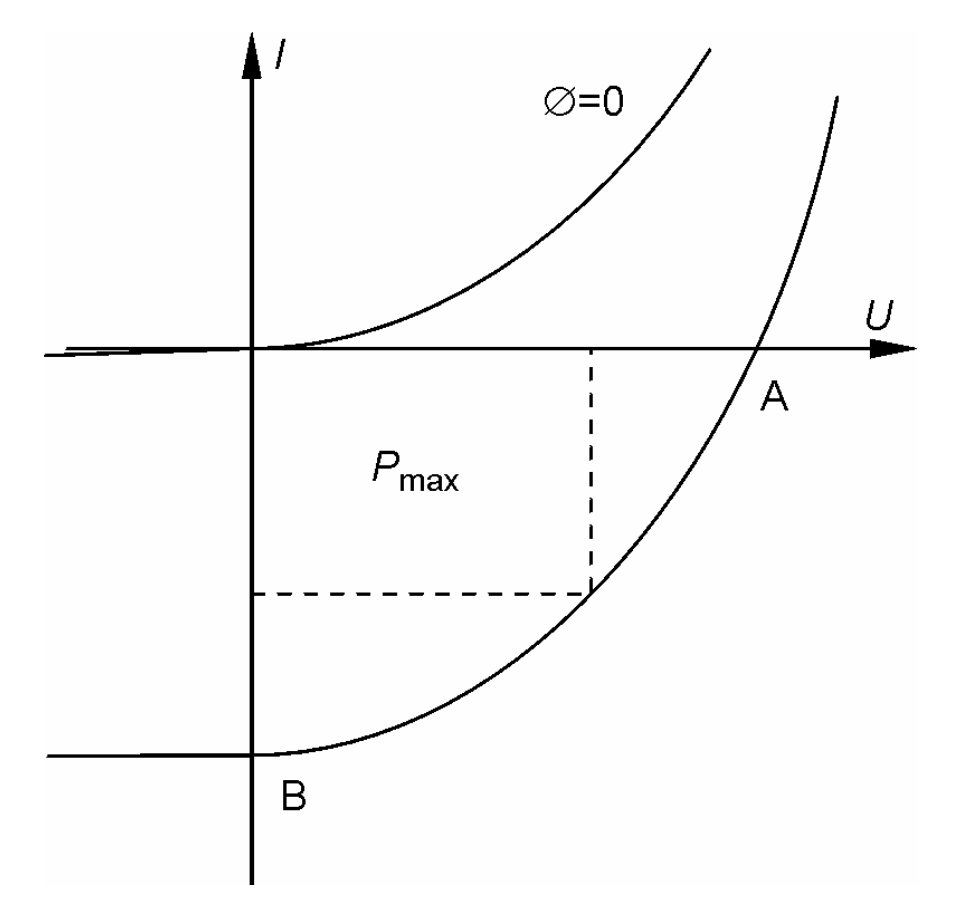
\includegraphics[width=0.3\linewidth]{image.png}
    \caption{
    Charakterystyki prądowo-napięciowe złącza p-n, ciemnego ($\Phi = 0$) i oświetlonego światłem (z zaznaczonym prostokątem mocy maksymalnej)}
    \label{fig:wykres-1}
\end{figure}

Charakterystyki prądowo-napięciowe ogniwa słonecznego przedstawia rysunek 1. Przy braku oświetlenia jest taka sama
jak zwykłej diody półprzewodnikowej. Analiza procesu konwersji światła słonecznego na energię elektryczną wskazuje, że maksymalna sprawność ogniwa krzemowego wynosi około 25\%. Budowane obecnie
ogniwa mają sprawność o połowę niższą

\section{Opis stanowiska i aparatury pomiarowej}
\begin{figure}[H]
    \centering
    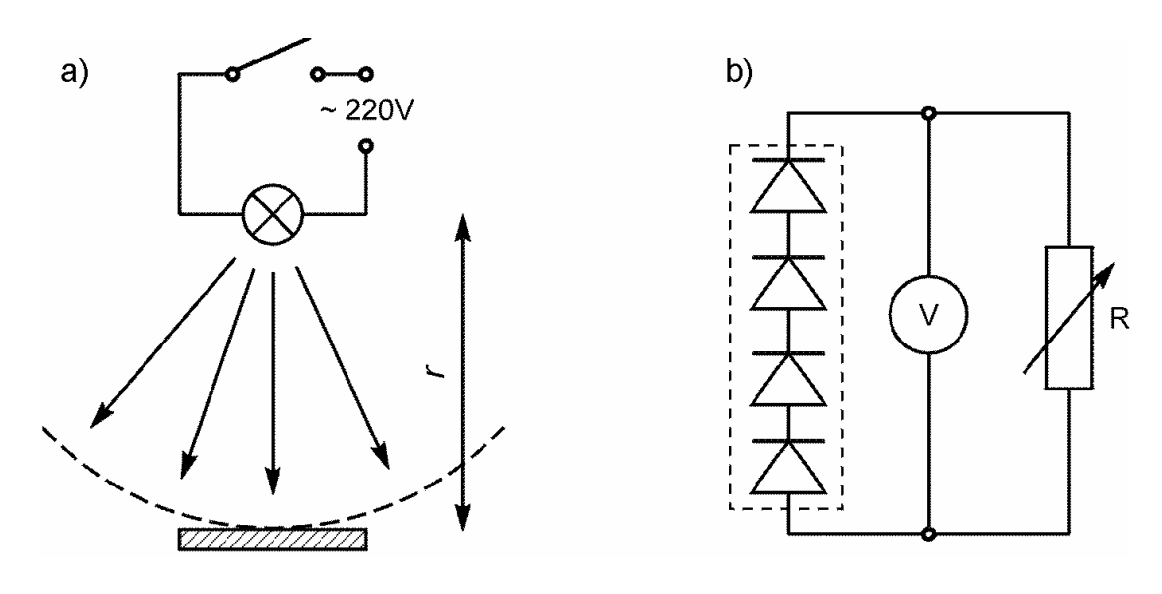
\includegraphics[width=0.5\linewidth]{aparatura_pomiarowa.png}
    \caption{Schemat układu eksperymentalnego: a) oświetlenie fotoogniwa lampą jarzeniową; b) układ elektryczny do badania charakterystyki prądowo-napięciowej }
\end{figure}

W skład układu pomiarowego wchodzą:
\begin{enumerate}
    \item Fotoogniwa krzemowe:
        \begin{itemize}
            \item monokrystaliczne
            \item polikrystaliczne
            \item amorficzne
        \end{itemize}
    \item Żarówka jarzeniowa o charakterystyce widmowej zbliżonej do światła dziennego.
    \item Woltomierz cyfrowy i miernik cyfrowy
\end{enumerate}

\section{Przebieg doświadczenia}
Po zestawieniu układu pomiarowego ustawiliśmy lampę w odległości około 25cm od ogniw.
Za pomocą luksomierza dokonaliśmy pomiary natężenia światła $\Phi$. Następnie wykonywaliśmy
pomiary mocy ogniwa dla trzech rodzajów ogniw.
Przeprowadziliśmy pomiary w całym dostępnym zakresie napięcia prądu.

\section{Wyniki pomiarów}

\begin{table}[H]
    \centering
    \caption{Parametry badanych ogniw.}
    \begin{tabular}{cccc}
        \thead{Typ ogniwa} &
        \thead{Liczba sekcji $n$ } & 
        \thead{Powierzchnia sekcji $S$ [$\text{cm}^2$] } &
        \thead{Powierzchnia całkowita $nS$ [$\text{cm}^2$]} \\ 
        \toprule
        Monokrystaliczne & 1  & 63 & 63 \\
        Polikrystaliczne & 8  & 7.8 & 62.4 \\
        Amorficzne & 14  & 5.5 & 77 \\
         
    \end{tabular}
    \label{tab:my_label}
\end{table}

Pomiaru natężenia światła wykonaliśmy przy użyciu elektronicznego luksomierza, 
\begin{equation*}
    \Phi = 56.3 \phiJ ; \quad
    u(\Phi) = 0.50  \phiJ
\end{equation*}

Przyjęliśmy niepewności równą $0.50 \phiJ$, z racji 
trudności w ustawieniu luksomierza w dokładnie takiej 
odległości i położeniu od lampy jak badane ogniwo.



Poniżej znajdują się tabele z wynikami
pomiarów. Zaznaczamy tutaj, że mierzone 
były jedynie kolumny $U$ i $I$, reszta 
kolumn jest obliczona przy użyciu tych
dwóch i parametrów poszczególnych ogniw.

\begin{table}[H]
    \caption{Wyniki pomiarów dla ogniwa monokrystalicznego}
    \centering
    \begin{tabular}{rrrrrr}
\toprule
$U$ [V] & $I$ [mA] & $P = U \cdot I$ [mW] & $R$ [$\Omega$] & $U/n$ [V] & $j=I/S$ [mA/$\text{cm}^2$] \\
\midrule
0.467 & -4.6 & 2.148 & 101.522 & 0.467 & 0.073 \\
0.465 & -4.8 & 2.232 & 96.875 & 0.465 & 0.076 \\
0.465 & -5.0 & 2.325 & 93.000 & 0.465 & 0.079 \\
0.465 & -5.3 & 2.464 & 87.736 & 0.465 & 0.084 \\
0.464 & -5.6 & 2.598 & 82.857 & 0.464 & 0.089 \\
0.464 & -6.0 & 2.784 & 77.333 & 0.464 & 0.095 \\
0.463 & -6.4 & 2.963 & 72.344 & 0.463 & 0.102 \\
0.462 & -6.9 & 3.188 & 66.957 & 0.462 & 0.110 \\
0.462 & -7.4 & 3.419 & 62.432 & 0.462 & 0.117 \\
0.461 & -8.1 & 3.734 & 56.914 & 0.461 & 0.129 \\
0.461 & -8.8 & 4.057 & 52.386 & 0.461 & 0.140 \\
0.461 & -9.8 & 4.518 & 47.041 & 0.461 & 0.156 \\
0.460 & -10.9 & 5.014 & 42.202 & 0.460 & 0.173 \\
0.458 & -12.3 & 5.633 & 37.236 & 0.458 & 0.195 \\
0.457 & -14.2 & 6.489 & 32.183 & 0.457 & 0.225 \\
0.455 & -16.8 & 7.644 & 27.083 & 0.455 & 0.267 \\
0.451 & -20.7 & 9.336 & 21.787 & 0.451 & 0.329 \\
0.446 & -25.9 & 11.551 & 17.220 & 0.446 & 0.411 \\
0.434 & -36.7 & 15.928 & 11.826 & 0.434 & 0.583 \\
0.390 & -57.0 & 22.230 & 6.842 & 0.390 & 0.905 \\
0.369 & -61.7 & 22.767 & 5.981 & 0.369 & 0.979 \\
0.340 & -66.1 & 22.474 & 5.144 & 0.340 & 1.049 \\
0.305 & -69.4 & 21.167 & 4.395 & 0.305 & 1.102 \\
0.273 & -71.3 & 19.465 & 3.829 & 0.273 & 1.132 \\
0.216 & -72.8 & 15.725 & 2.967 & 0.216 & 1.156 \\
0.148 & -73.3 & 10.848 & 2.019 & 0.148 & 1.163 \\
0.118 & -73.5 & 8.673 & 1.605 & 0.118 & 1.167 \\
\bottomrule
\end{tabular}

\end{table}

\begin{table}[H]
    \centering
    \caption{Wyniki pomiarów dla ogniwa polikrystalicznego.}
\begin{tabular}{rrrrrr}
\toprule
$U$ [V] & $I$ [mA] & $P = U \cdot I$ [mW] & $R$ [$\Omega$] & $U/n$ [V] & $j=I/S$ [mA/$\text{cm}^2$] \\
\midrule
2.725 & -1.35 & 3.679 & 2018.519 & 0.341 & 0.173 \\
2.711 & -1.42 & 3.850 & 1909.155 & 0.339 & 0.182 \\
2.698 & -1.48 & 3.993 & 1822.973 & 0.337 & 0.190 \\
2.683 & -1.56 & 4.185 & 1719.872 & 0.335 & 0.200 \\
2.669 & -1.64 & 4.377 & 1627.439 & 0.334 & 0.210 \\
2.654 & -1.74 & 4.618 & 1525.287 & 0.332 & 0.223 \\
2.637 & -1.84 & 4.852 & 1433.152 & 0.330 & 0.236 \\
2.616 & -1.96 & 5.127 & 1334.694 & 0.327 & 0.251 \\
2.592 & -2.11 & 5.469 & 1228.436 & 0.324 & 0.271 \\
2.563 & -2.27 & 5.818 & 1129.075 & 0.320 & 0.291 \\
2.526 & -2.47 & 6.239 & 1022.672 & 0.316 & 0.317 \\
2.486 & -2.66 & 6.613 & 934.586 & 0.311 & 0.341 \\
2.431 & -2.94 & 7.147 & 826.871 & 0.304 & 0.377 \\
2.394 & -3.10 & 7.421 & 772.258 & 0.299 & 0.397 \\
2.351 & -3.28 & 7.711 & 716.768 & 0.294 & 0.421 \\
2.320 & -3.40 & 7.888 & 682.353 & 0.290 & 0.436 \\
2.261 & -3.63 & 8.207 & 622.865 & 0.283 & 0.465 \\
2.213 & -3.82 & 8.454 & 579.319 & 0.277 & 0.490 \\
2.132 & -4.09 & 8.720 & 521.271 & 0.267 & 0.524 \\
2.020 & -4.43 & 8.949 & 455.982 & 0.253 & 0.568 \\
1.909 & -4.72 & 9.010 & 404.449 & 0.239 & 0.605 \\
1.709 & -5.12 & 8.750 & 333.789 & 0.214 & 0.656 \\
1.420 & -5.51 & 7.824 & 257.713 & 0.177 & 0.706 \\
1.088 & -5.73 & 6.234 & 189.878 & 0.136 & 0.735 \\
0.727 & -5.88 & 4.275 & 123.639 & 0.091 & 0.754 \\
0.340 & -5.98 & 2.033 & 56.856 & 0.043 & 0.767 \\
0.067 & -6.02 & 0.403 & 11.130 & 0.008 & 0.772 \\
\bottomrule
\end{tabular}
\end{table}

\begin{table}[H]
    \centering
    \caption{Wyniki pomiarów dla ogniwa amorficznego.}
\begin{tabular}{rrrrrr}
\toprule
$U$ [V] & $I$ [mA] & $P = U \cdot I$ [mW] & $R$ [$\Omega$] & $U/n$ [V] & $j=I/S$ [mA/$\text{cm}^2$] \\
\midrule
9.735 & -0.50 & 4.868 & 19470.000 & 0.695 & 0.091 \\
9.695 & -0.52 & 5.041 & 18644.231 & 0.693 & 0.095 \\
9.678 & -0.55 & 5.323 & 17596.364 & 0.691 & 0.100 \\
9.638 & -0.62 & 5.976 & 15545.161 & 0.688 & 0.113 \\
9.588 & -0.70 & 6.712 & 13697.143 & 0.685 & 0.127 \\
9.520 & -0.82 & 7.806 & 11609.756 & 0.680 & 0.149 \\
9.420 & -0.97 & 9.137 & 9711.340 & 0.673 & 0.176 \\
9.255 & -1.20 & 11.106 & 7712.500 & 0.661 & 0.218 \\
9.120 & -1.37 & 12.494 & 6656.934 & 0.651 & 0.249 \\
8.926 & -1.57 & 14.014 & 5685.350 & 0.638 & 0.285 \\
8.623 & -1.84 & 15.866 & 4686.413 & 0.616 & 0.335 \\
8.055 & -2.17 & 17.479 & 3711.982 & 0.575 & 0.395 \\
6.728 & -2.47 & 16.618 & 2723.887 & 0.481 & 0.449 \\
6.250 & -2.52 & 15.750 & 2480.159 & 0.446 & 0.458 \\
5.407 & -2.57 & 13.896 & 2103.891 & 0.386 & 0.467 \\
4.877 & -2.60 & 12.680 & 1875.769 & 0.348 & 0.473 \\
4.389 & -2.62 & 11.499 & 1675.191 & 0.314 & 0.476 \\
3.818 & -2.63 & 10.041 & 1451.711 & 0.273 & 0.478 \\
3.275 & -2.65 & 8.679 & 1235.849 & 0.234 & 0.482 \\
2.519 & -2.67 & 6.726 & 943.446 & 0.180 & 0.485 \\
1.887 & -2.68 & 5.057 & 704.104 & 0.135 & 0.487 \\
1.284 & -2.71 & 3.480 & 473.801 & 0.092 & 0.493 \\
0.678 & -2.72 & 1.844 & 249.265 & 0.048 & 0.495 \\
0.058 & -2.74 & 0.159 & 21.168 & 0.004 & 0.498 \\
0.044 & -2.72 & 0.120 & 16.176 & 0.003 & 0.495 \\
\bottomrule
\end{tabular}
\end{table}

\section{Opracowanie wyników}
\subsection{Badanie charakterystyki prądowo-napięciowej.}

Charakterystyka prądowo-napięciowa fotoogniwa według teorii wyraża się wzorem:
\begin{equation*}
    I = I_s \left[ \exp \left(  \frac{eU}{mkT} \right) -1 \right] - \text{const} \cdot \Phi
\end{equation*}

Zatem wykresy $I = f(U)$ dla poszczególnych ogniw powinny przyjmować
kształt krzywej wykładniczej: $y = a e^{bx} + c$, by to sprawdzić
rysujemy wykres $I = f(U)$ dla każdego ogniwa , a następnie
dopasowujemy krzywą wykładniczą.


\begin{figure}[H]
    \centering
    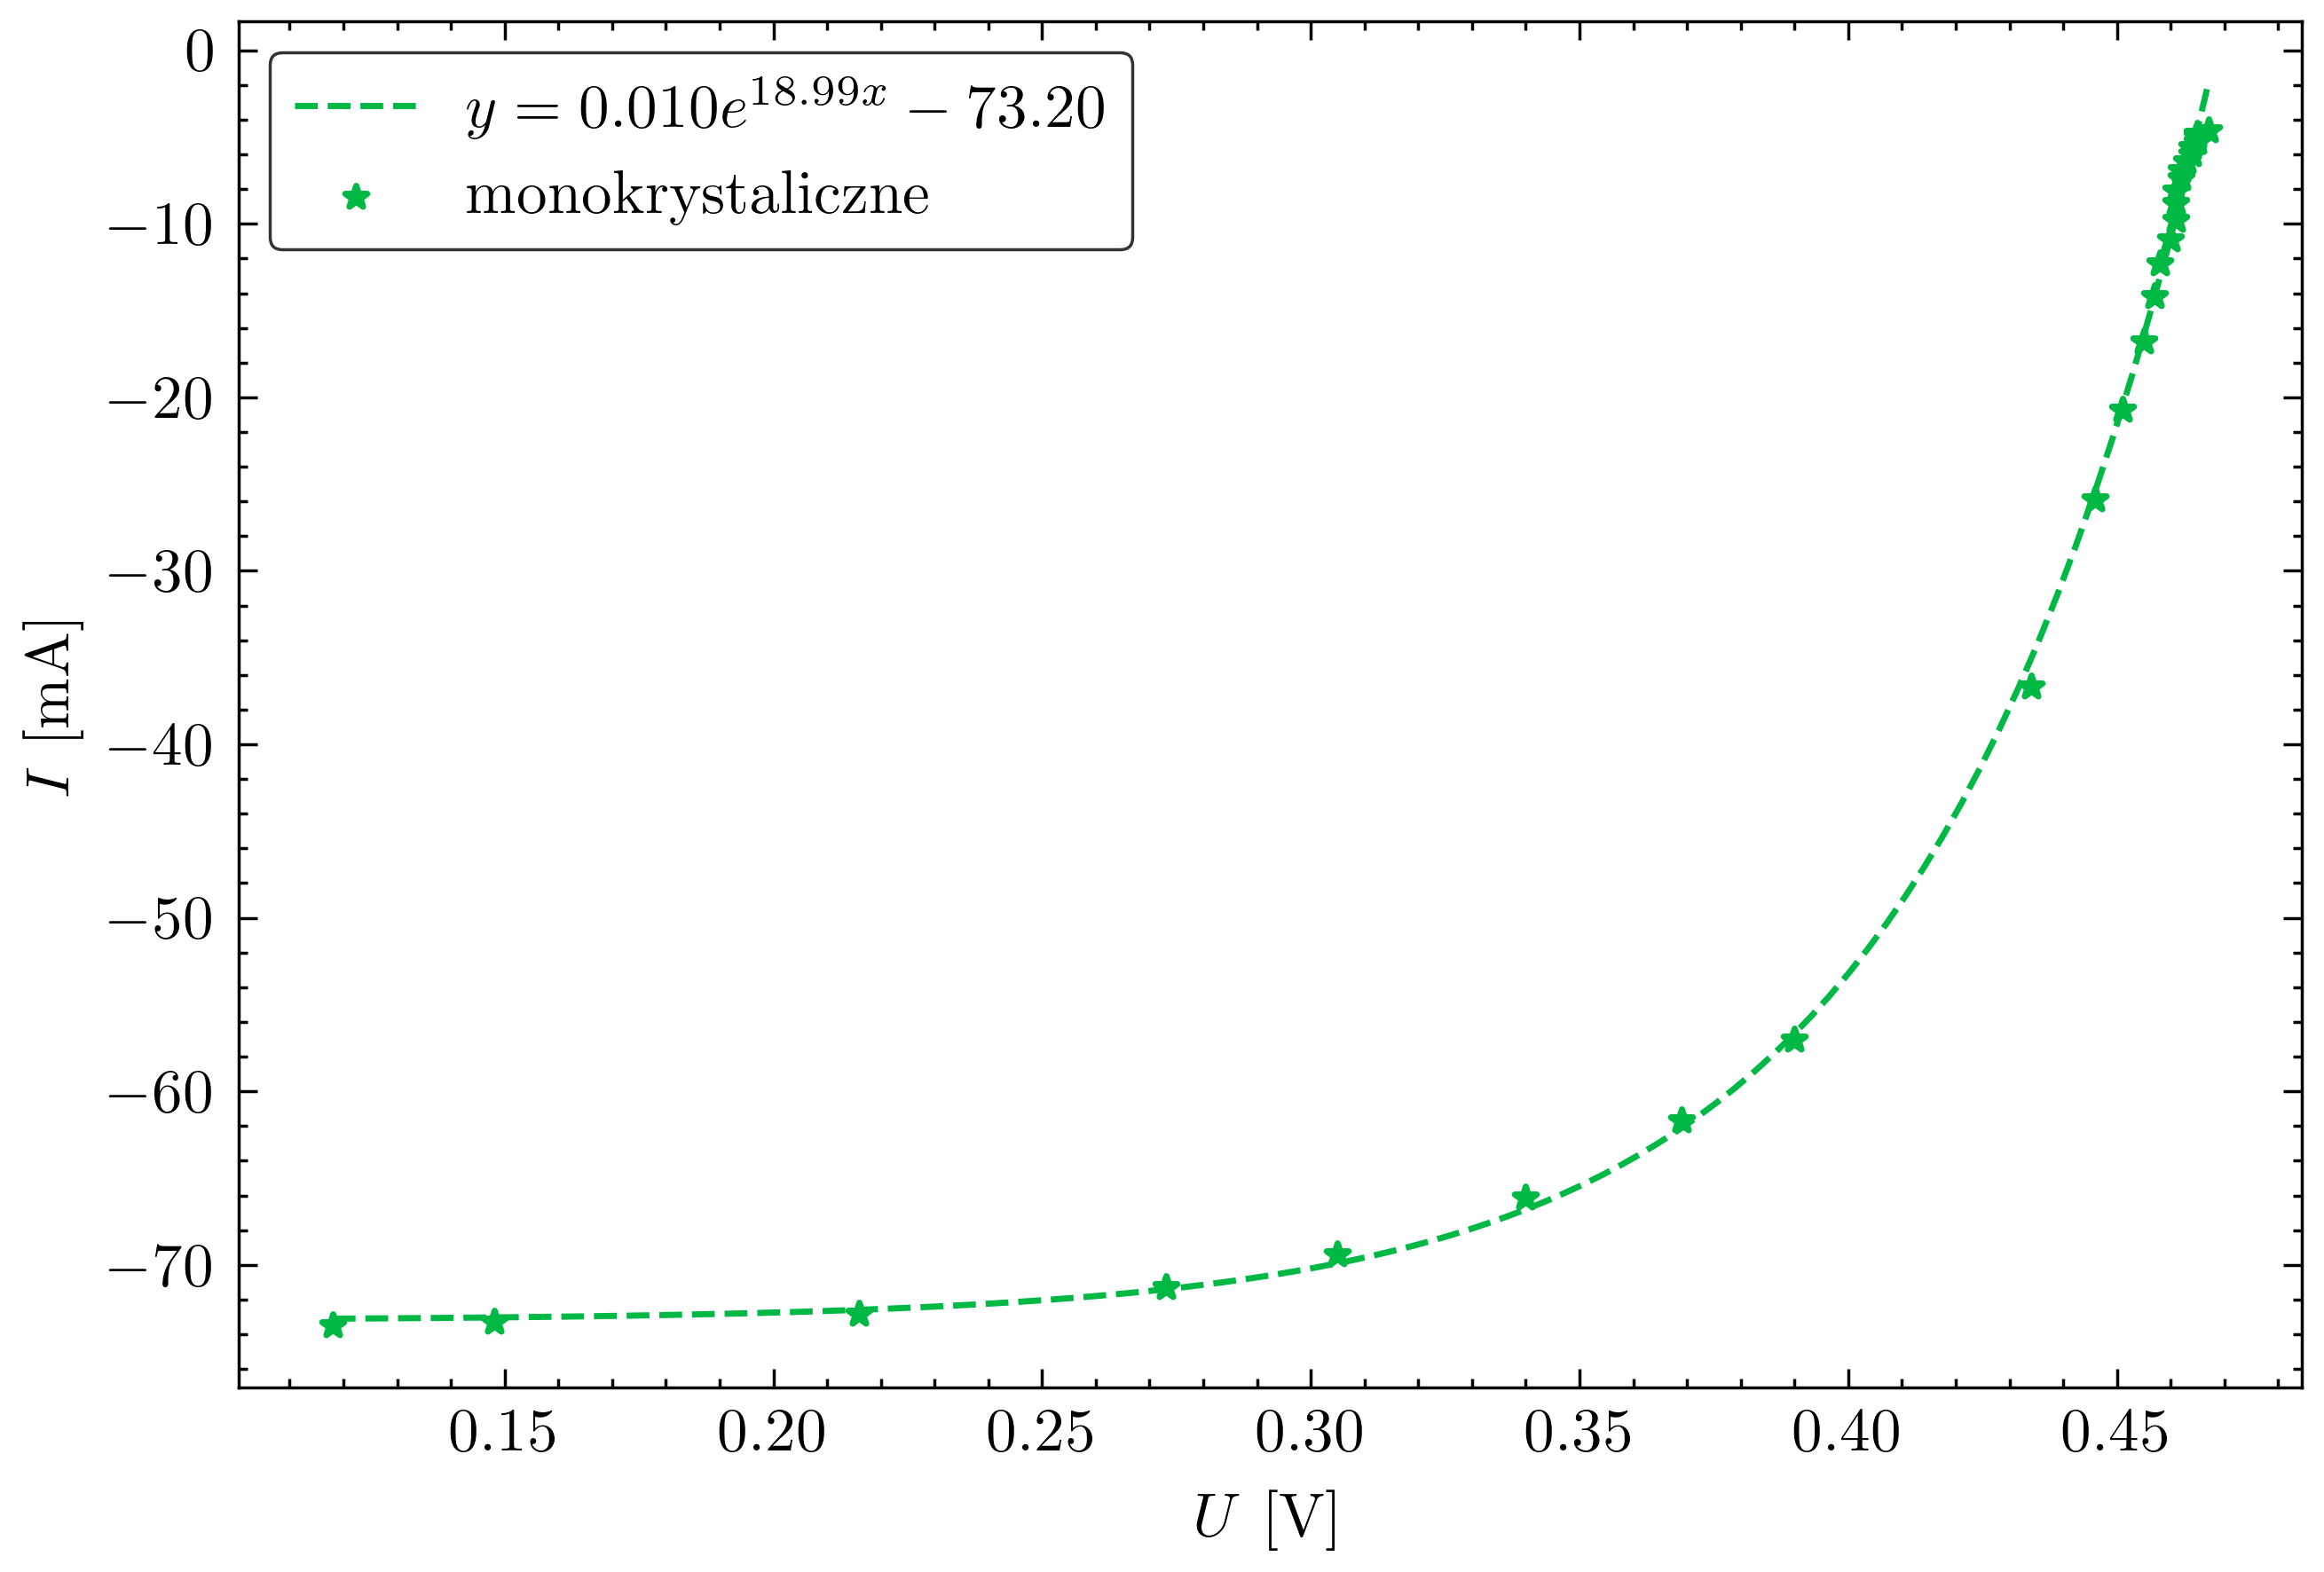
\includegraphics[width=0.7\linewidth]{mono.png}
    \caption{
    Charakterystyka prądowo-napięciowa dla ogniwa monokrystalicznego z dopasowaną
    krzywą wykładniczą.}
\end{figure}

\begin{figure}[H]
    \centering
    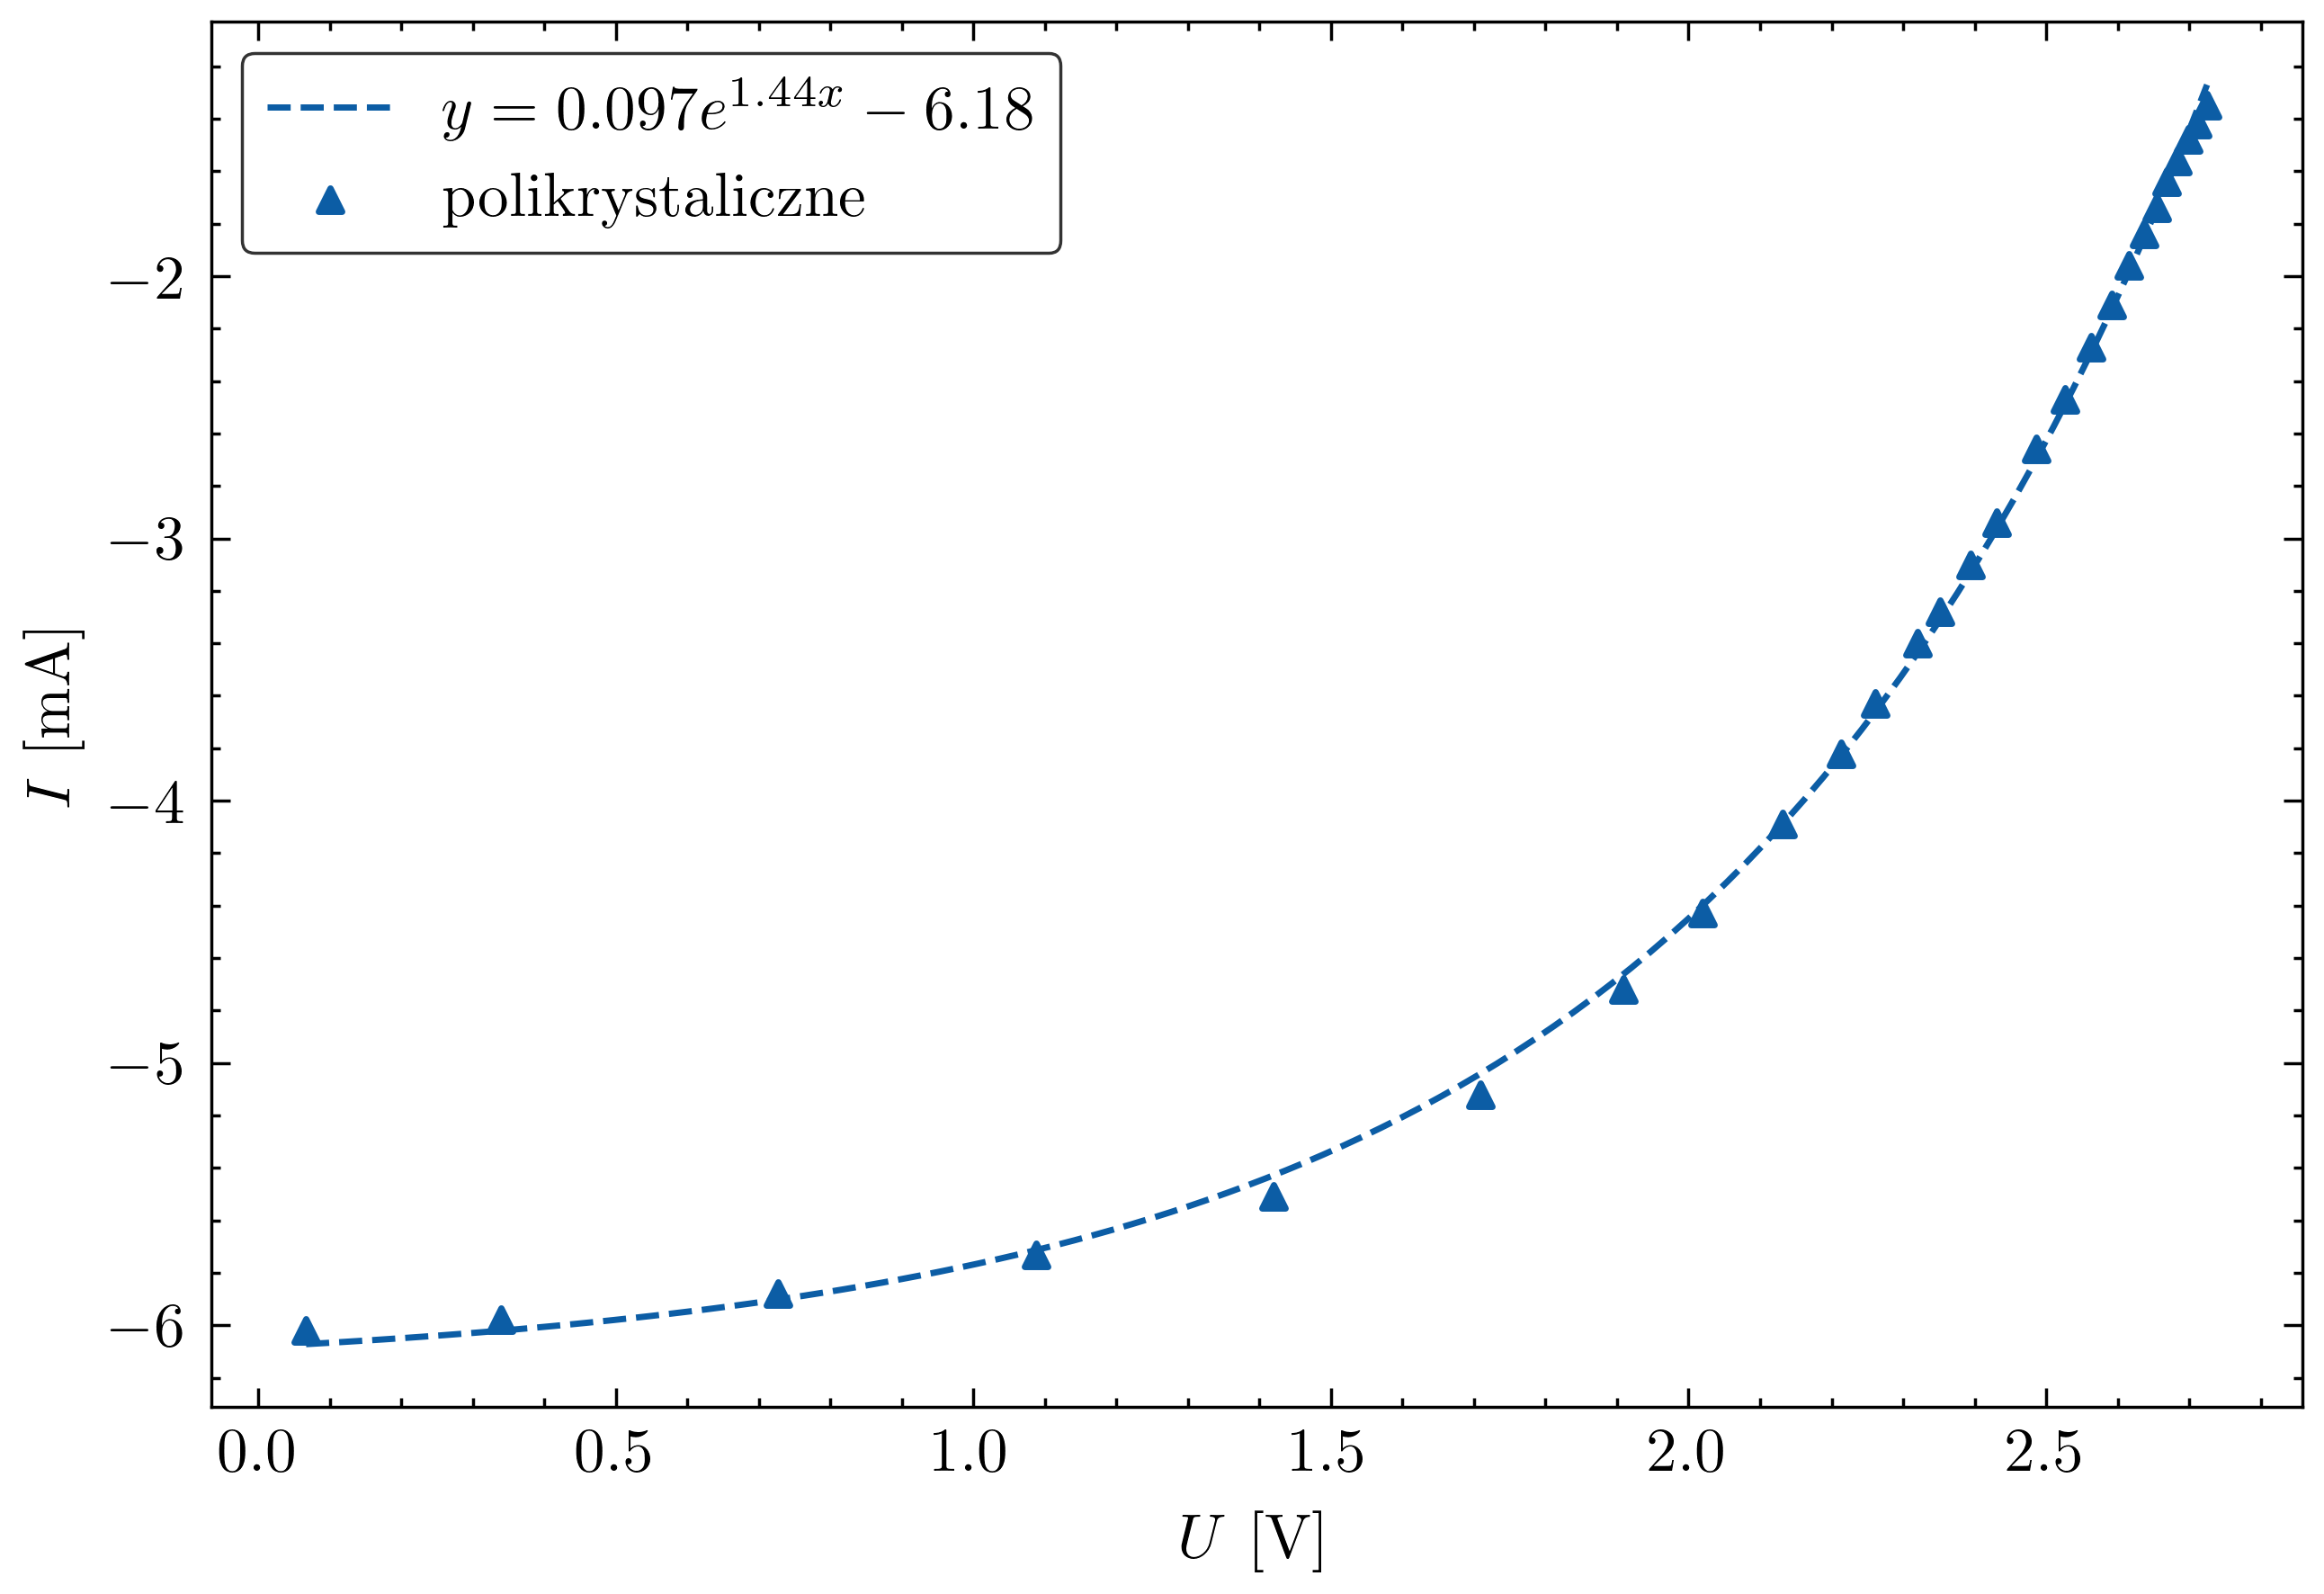
\includegraphics[width=0.7\linewidth]{poli.png}
    \caption{
    Charakterystyka prądowo-napięciowa dla ogniwa polikrystalicznego z dopasowaną
    krzywą wykładniczą.}
\end{figure}

\begin{figure}[H]
    \centering
    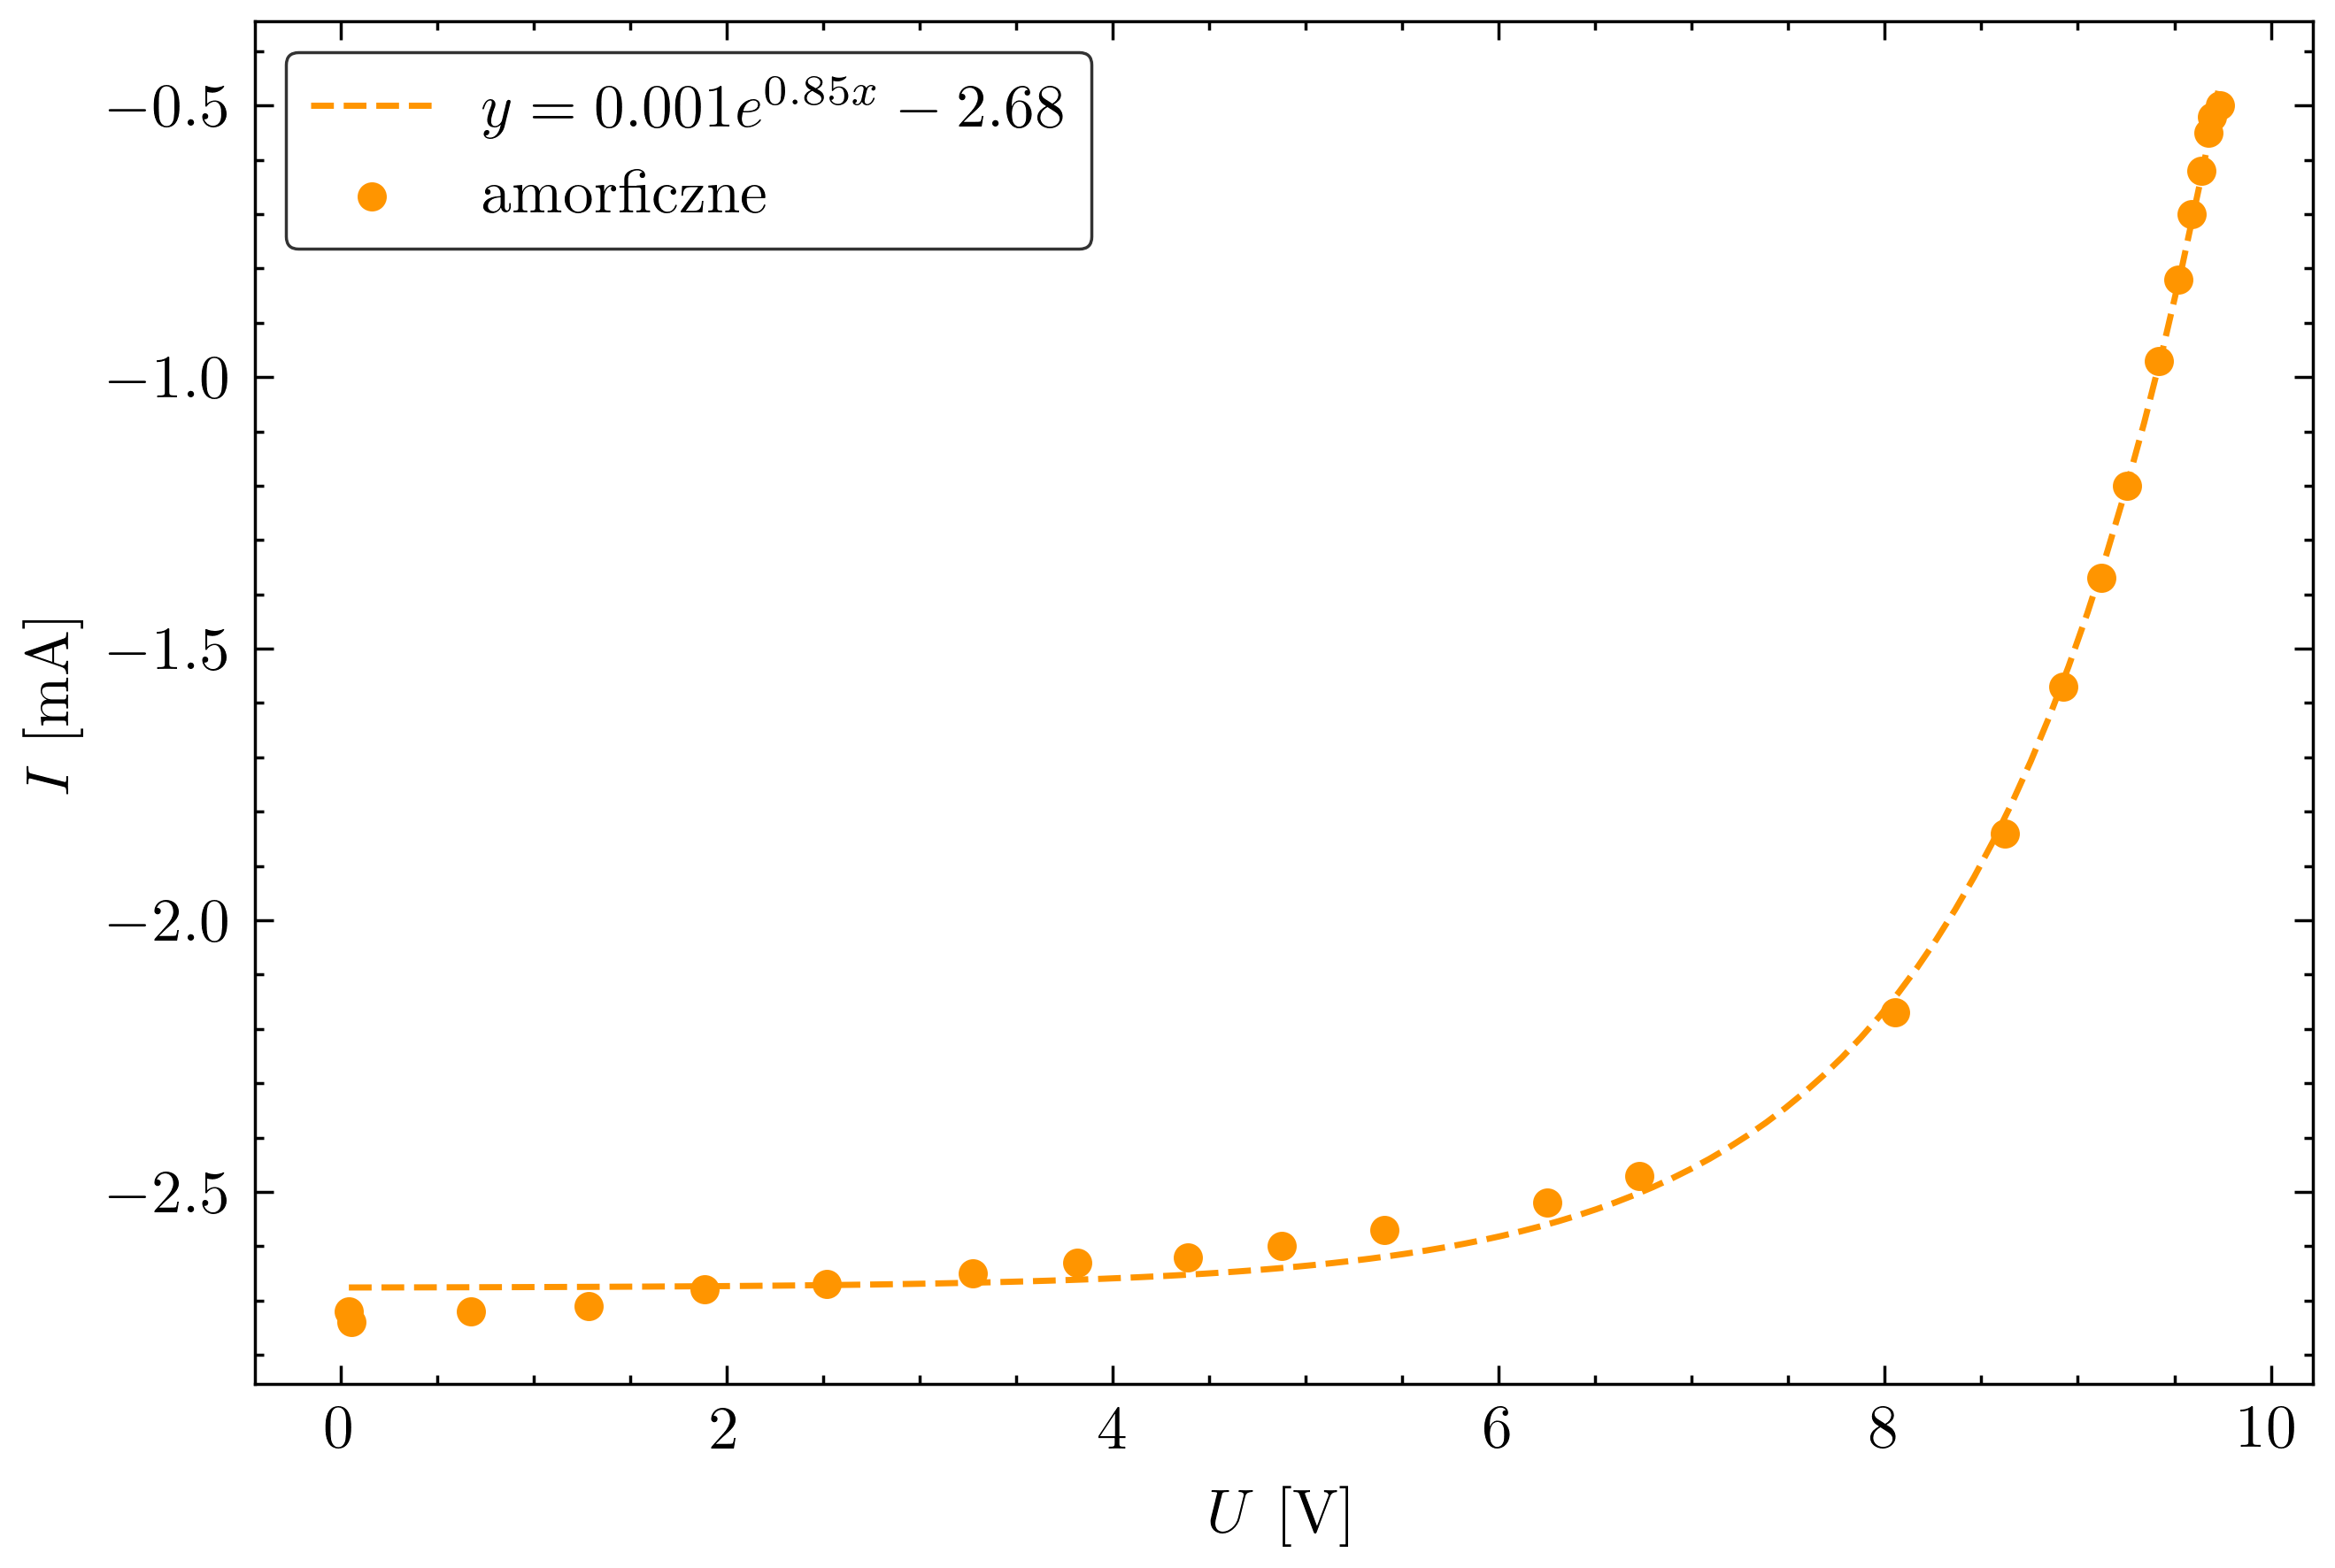
\includegraphics[width=0.7\linewidth]{amorf.png}
    \caption{
    Charakterystyka prądowo-napięciowa dla ogniwa amorficznego z dopasowaną
    krzywą wykładniczą.}
\end{figure}

W celu porównania charakterystyk pomiędzy fotoogniwami wykonujemy
wspólny wykres $I/S = f(U/n)$.

\begin{figure}[H]
    \centering
    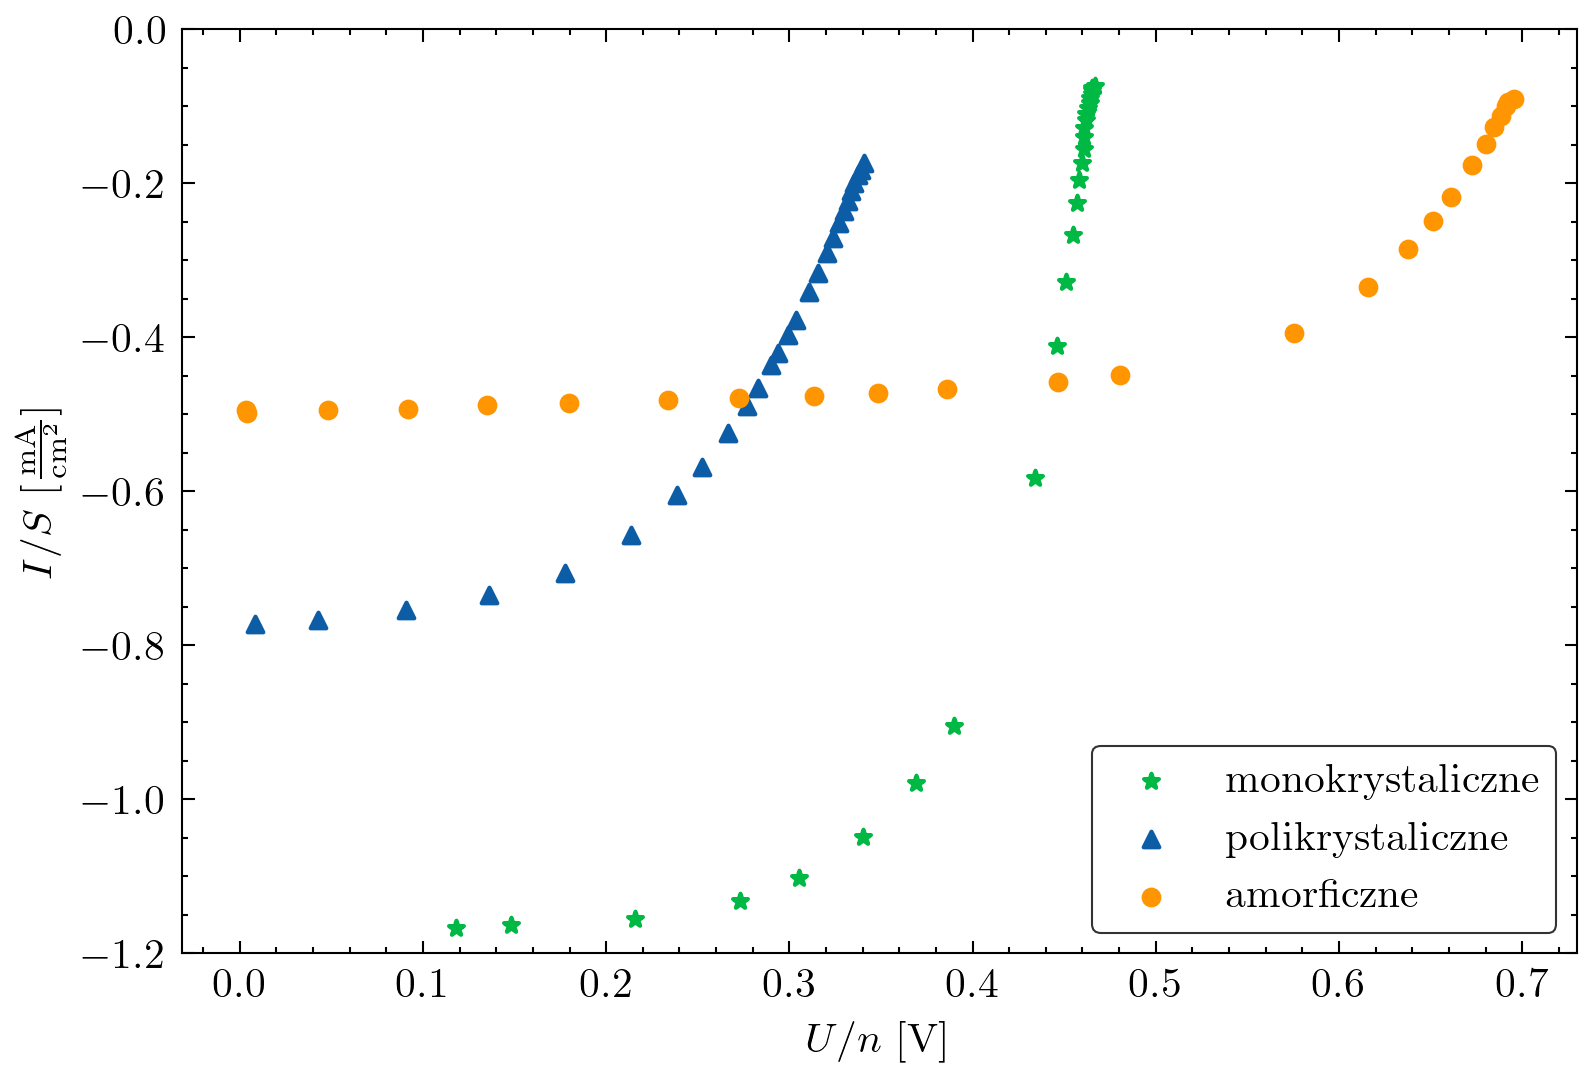
\includegraphics[width=0.7\linewidth]{combined.png}
    \caption{
        Wspólny wykres znormalizowanych charakterystyk: $I/S = f(U/n)$
    }
\end{figure}

\subsection{Sprawność ogniw}
By obliczyć sprawność ogniwa potrzebujemy mocy maksymalnej. 
Moc maksymalną dla każdego fotoogniwa możemy odczytać z tabeli pomiarów.
Uznajemy, że
\begin{itemize}
    \item dla ogniwa polikrystalicznego i amorficznego $u(U) = 0.01 \volt; \; U(I) = 0.02 \mampr$
    \item dla ogniwa monokrystalicznego $u(U) = 0.01 \volt;\; U(I) = 0.1 \mampr$,
    niepewność $I$ uznajemy za większą w porównaniu z innymi fotoogniwami, 
    ponieważ musieliśmy użyć szerszego zakresu badając to ogniwo.
\end{itemize}
Wybraliśmy takie niepewności z racji wahań przyrządów pomiarowych.

Niepewność $P_\text{max}$  obliczamy z prawa przenoszenia niepewności:
\begin{equation*}
    u(P_\text{max}) = \sqrt{
    \left[ \frac{\partial P_\text{max}}{\partial I} \cdot u(I) \right]^2 + 
    \left[ \frac{\partial P_\text{max}}{\partial U} \cdot u(U) \right]^2
    } = \sqrt{
    \left[ U \cdot u(I) \right]^2 + 
    \left[ I \cdot u(U) \right]^2
    }
\end{equation*}

Sprawność ogniwa wyraża się wzorem:
\begin{equation*}
    \eta = \frac{P_\text{max}}{\Phi n S}
\end{equation*}

Zatem jej niepewność to :
\begin{equation*}
    u(\eta) = \sqrt {
        \left[ \frac{\partial \eta}{\partial P_\text{max}} u(P_\text{max}) \right]^2 +
        \left[ \frac{\partial \eta}{\partial \Phi} u(\Phi) \right]^2
    } = \sqrt {
        \left[ \frac{1}{\Phi n S} u(P_\text{max}) \right]^2 +
        \left[ \frac{-P_\text{max}}{\Phi^2 nS} u(\Phi) \right]^2
    } 
\end{equation*}

Zatem dla ogniwa monokrystalicznego:
\begin{align*}
    P_\text{max} &= 22.767 \mwat \\
    U &= 0.369 \volt \\
    I &= 61.7 \mampr \\
    \eta &= \frac{22.767 \mwat}{56.3 \phiJ \cdot 63 \text{cm}^2} = 6.4188 \% \\
    u(P_\text{max}) &=  \sqrt{
    \left( 0.369 \volt \cdot 0.1 \mampr \right)^2 + 
    \left( 61.7 \mampr \cdot 0.01 \volt \right)^2
    } = 0.62 \mwat  \\
    u(\eta) &= \sqrt {
        \left( \frac{1}{56.3 \phiJ \cdot 63 \text{cm}^2 } \cdot 0.62 \mwat \right)^2 +
        \left( \frac{-22.767 \mwat}{ \left(56.3 \phiJ\right)^2 \cdot 63 \text{cm}^2}
        \cdot 0.5 \phiJ \right)^2
    } = 0.19 \%
\end{align*}


Dla ogniwa polikrystalicznego:
\begin{align*}
    P_\text{max} &= 9.010 \mwat \\
    U &= 1.909 \volt \\
    I &= 4.72 \mampr \\
    \eta &= \frac{9.010 \mwat}{56.3 \phiJ \cdot 62.4 \text{cm}^2} = 2.5648 \% \\
    u(P_\text{max}) &=  \sqrt{
    \left( 1.909 \volt \cdot 0.02 \mampr \right)^2 + 
    \left( 4.72 \mampr \cdot 0.01 \volt \right)^2
    } = 0.061 \mwat  \\
    u(\eta) &= \sqrt {
        \left( \frac{1}{56.3 \phiJ \cdot 62.4 \text{cm}^2 } \cdot 0.061 \mwat \right)^2 +
        \left( \frac{-9.010 \mwat}{ \left(56.3 \phiJ\right)^2 \cdot 62.4 \text{cm}^2}
        \cdot 0.5 \phiJ \right)^2
    } = 0.029 \%
\end{align*}


Dla ogniwa amorficznego:
\begin{align*}
    P_\text{max} &= 17.479 \mwat \\
    U &= 8.055 \volt \\
    I &= 2.17 \mampr \\
    \eta &= \frac{17.479 \mwat}{56.3 \phiJ \cdot 77 \text{cm}^2} = 4.0320 \% \\
    u(P_\text{max}) &=  \sqrt{
    \left( 8.055 \volt \cdot 0.02 \mampr \right)^2 + 
    \left( 2.17 \mampr \cdot 0.01 \volt \right)^2
    } = 0.17 \mwat  \\
    u(\eta) &= \sqrt {
        \left( \frac{1}{56.3 \phiJ \cdot 77 \text{cm}^2 } \cdot 0.17 \mwat \right)^2 +
        \left( \frac{-17.479 \mwat}{ \left(56.3 \phiJ\right)^2 \cdot 77 \text{cm}^2}
        \cdot 0.5 \phiJ \right)^2
    } = 0.052 \%
\end{align*}

Wyniki naszych obliczeń przedstawiamy w postaci tabeli:

\begin{table}[H]
    \centering
    \caption{Moc maksymalna oraz sprawności dla poszczególnych ogniw}
    \begin{tabular}{ccccc}
        \thead{Typ ogniwa} &
        $P_\text{max}$ [$\text{mW}$] & 
        $u(P_\text{max})$ [$\text{mW}$]  &
        $\eta$ [\%] & 
        $u(\eta)$ [\%] \\
        \toprule
        Monokrystaliczne & $22.77 \mwat$ & $0.62 \mwat$ & $6.42 \%$ & $0.19 \%$ \\
        Polikrystaliczne & $ 9.010 \mwat$ & $0.061 \mwat$ & $2.565 \%$ & $0.029 \%$ \\
        Amorficzne & $ 17.48 \mwat$ & $0.17 \mwat$ & $4.032 \%$ & $0.052 \%$ \\
    \end{tabular}
\end{table}

Największą sprawność posiada ogniwo monokrystaliczne wynoszące $6.42 \%$.
Otrzymane wartości sprawności ogniw są niższe, niż przewidywane.
Ogniwa monokrystaliczne uzyskując sprawność od 16 \% do  22 \%.
Może to być spowodowane: wadami badanego układu, zanieczyszczeniom
na powierzchni ogniw lub złym pomiarem natężenia światła.
Warto zwrócić uwagę na fakt, iż doświadczenie było wykonywane w dużej sali
fizycznej gdzie otaczające światło mogło się często zmieniać.




\subsection{Gęstość prądu zwarcia oraz napięcie przypadające na sekcję}

\begin{table}[H]
    \centering
    \caption{Gęstość prądu zwarcia oraz napięcie przypadające na sekcję
            dla poszczególnych rodzajów ogniw.
    }
    \begin{tabular}{ccc}
        \thead{Typ ogniwa} &
        $j=\frac{I}{S}$ [$\frac{\text{mA}}{\text{cm}^2}$] & 
        $\frac{U}{n}$ [$\text{V}$]  \\
        \toprule
        Monokrystaliczne & 0.979 & 0.369 \\
        Polikrystaliczne & 0.605& 0.239  \\
        Amorficzne & 0.395 & 0.575 \\
    \end{tabular}
\end{table}

Ogniwo monokrystaliczne posiada największą gęstość prądu zwarcia,
a ogniwo amorficzne ma największe  napięcie przypadające na sekcję.

\newpage
\section{Wnioski}
W wyniku doświadczenia obliczyliśmy sprawności różnych 
trzech różnych rodzajów fotoogniw.
Otrzymane sprawności ogniw są niższe niż przewidywane (monokrystaliczne uzyskują
zazwyczaj sprawność od 16\% do 22\% - u nas w doświadczeniu 6.42\%). 
Może to być spowodowane wadami badanego układu,
zanieczyszczeniom na powierzchni ogniw lub złym pomiarem natężenia światła.
Z naszych obliczeń wynika, że największą sprawność spośród badanych ogniw ma ogniwo monokrystaliczne.

Posiada ono również najwyższą gęstość prądu zwarcia. Ogniwo amorficzne ma natomiast
największe napięcie przypadające na sekcję.

Używając otrzymanych pomiarów stworzyliśmy wykresy zależności $I = f(U)$.
Zgodnie z przewidywaniami wykresy te przyjmują kształt krzywej wykładniczej.


\end{document}
 
 
 

